\documentclass[a4j]{jarticle}
\usepackage{ascmac}
\usepackage{comment}
\usepackage{url}
\usepackage[dvipdfmx]{graphicx}
\usepackage{listings,jvlisting, jlisting}

\lstset{
  basicstyle={\ttfamily},
  identifierstyle={\small},
  commentstyle={\smallitshape},
  keywordstyle={\small\bfseries},
  ndkeywordstyle={\small},
  stringstyle={\small\ttfamily},
  frame={tb},
  breaklines=true,
  columns=[l]{fullflexible},
  numbers=left,
  xrightmargin=0zw,
  xleftmargin=3zw,
  numberstyle={\scriptsize},
  stepnumber=1,
  numbersep=1zw,
  lineskip=-0.5ex
}

\begin{document}

\vfill
\begin{screen}
  \begin{center}
    \huge\bf 実験　レポート1\\
    \vspace{5mm}
    \large\bf
    学籍番号　2022311042 \ 名前 神野友哉\\
    \today
  \end{center}
\end{screen}
\thispagestyle{empty}
%%目次
\tableofcontents

\newpage
% "%"同士に挟まれた行に書けばいいよ
\section{実験}
%
情報科学実験 1 の前期\ 4\ ～\ 7\ 週\quad 3DCG製作実験
%
\subsection{目的}
%
実験の目的は、基礎的な3DCG技術および、専門用語の造詣を深めること。
%
\subsection{方法や条件}
%
演習室の\ PC\ にて、3ds\ MAX\ というソフトウェアの教育版を利用する。
%
\subsection{結果}
%
目的は概ね達成された。操作方法や全体から見たごく一部の機能を、実際に用いることで学ぶことが出来た。
%
\subsection{考察}
%
周囲の学生と頻繁に知恵を共有したことが、結果的に効率的に学習を進められた要因だと考えられる。
%
\subsection{講義時間以外の取り組み時間}
%
実験自体は\ 2\ ～\ 3\ 時間、レポート作成込みで\ 6\ 時間程度
%
\subsection{自己評価}
%
S
%


\newpage
\section{課題\ 1}
1.3.1節で作成したロボットに新たに可動部品を追加し、レンダリングしなさい。ただし、まだ紹介されていない3ds\ Max\ の機能を\ 2\ つ以上利用すること
\subsection{考察}
%
以下の図\ref{fig:d} を製作することが出来た。新しく追加した可動部品としては、頭部上の王冠と、両肩に翼を模した板である。
課題を実施した際、基点移動に困らされる事が多かった。具体的には、ある平面画面では調整完了しても、俯瞰視点では、
離れた位置に調整されていたことや、基点移動対象ではない部位を選択していたことである。
それでも、基点移動のコツを習得することが出来た。それは、二つの互いに垂直な平面画面を活用することである。
平面はさいころをクリックする事で調整が可能であり、双方画面に表示される基点位置を目標位置に移動する。
こうして、基点位置を少ない移動回数で移動できる。
また、左翼は右翼の複製であり、パラメータは共通していて図\ref{fig:kRt}となっている。
%



% 下のコードで画像を二枚組にする。newpage は任意
\begin{figure}[htbp]
  \begin{minipage}{0.5\hsize}
    \begin{center}
      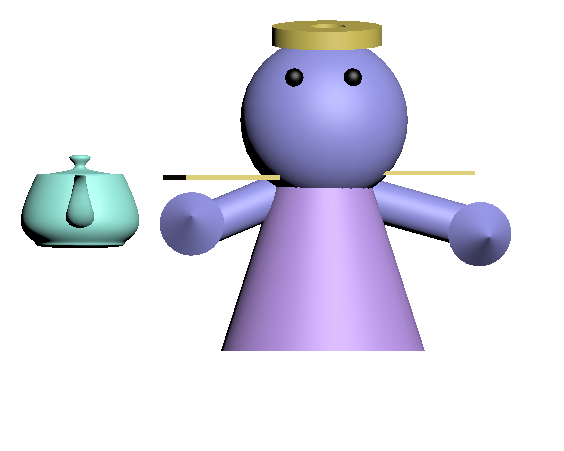
\includegraphics[width=70mm, height=50mm]{no/mydoll.png}
    \end{center}
    \caption{mydoll.png}
    \label{fig:d}
  \end{minipage}
  \begin{minipage}{0.5\hsize}
    \begin{center}
      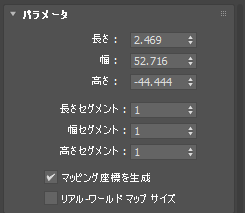
\includegraphics[width=70mm, height=50mm]{no/kataR-t.png}
    \end{center}
    \caption{wingR.png}
    \label{fig:kRt}
  \end{minipage}
\end{figure}

図\ref{fig:kkLt}, \ref{fig:kkRt}の基点は首の周りに調整されている。

\begin{figure}[htbp]
  \begin{minipage}{0.5\hsize}
    \begin{center}
      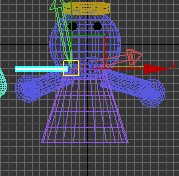
\includegraphics[width=70mm, height=50mm]{no/kitenkataL-t.png}
    \end{center}
    \caption{kwingL.png}
    \label{fig:kkLt}
  \end{minipage}
  \begin{minipage}{0.5\hsize}
    \begin{center}
      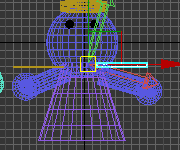
\includegraphics[width=70mm, height=50mm]{no/kitenkataR-t.png}
    \end{center}
    \caption{kwingR.png}
    \label{fig:kkRt}
  \end{minipage}
\end{figure}

\newpage
図\ref{fig:ct}は王冠のパラメータである。

\begin{figure}[htbp]
  \begin{minipage}{0.5\hsize}
    \begin{center}
      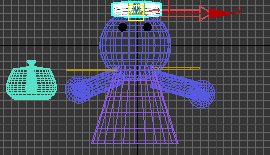
\includegraphics[width=70mm, height=50mm]{no/kitencrown-t.png}
    \end{center}
    \caption{kc.png}
    \label{fig:kct}
  \end{minipage}
  \begin{minipage}{0.5\hsize}
    \begin{center}
      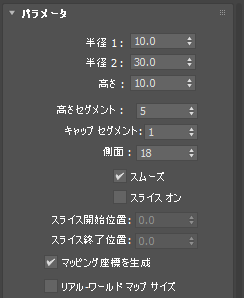
\includegraphics[width=70mm, height=50mm]{no/crown-t.png}
    \end{center}
    \caption{c.png}
    \label{fig:ct}
  \end{minipage}
\end{figure}

\newpage
\section{課題\ 2}
課題\ 1 \ で利用した\ 3ds\ Max\ の機能について、その特徴、役割、操作方法などを解説しなさい。
\subsection{考察}
%
翼では\ Box\ を、王冠では\ Tube\ を用いた。
前者は、縦、横、高さ等を指定して直方体を作成できる。その立体自体の汎用性によって、\ 3\ DCG作成に使われる頻度は比較的高い
と考えられる。各頂点周辺を切り取りや、引き延ばし、面によって色を塗る等も可能である。
後者は、外円半径、内円半径、高さ等を指定して、ストローや導管等に用いられる円筒を作成できる。
円柱\ Cylinder\ との差別点は、空洞となる内円部分の半径をパラメータで指定することで、操作し易い点である。
%

\newpage
\section{課題\ 3}
この実験では人間が手作業で行う\ CG\ 制作を体験しているが、最近では生成系\ AI\ を利用して\ CG\ を製作することも盛んに行われている。人間が手作業で行う\ CG\ 製作と生成系\ AI\ が作成する
\ CG\ を比較して、人間でなければ作成できない部分、人間では作成できない部分について述べなさい。
\subsection{考察}
%
ウェブサイトAismileyによると、AIの強みは膨大なデータを素早く処理でき、類似の作業を高速かつ一貫して実行できるという\cite{Aismiley}。
これにより、多くのコンテンツを短時間で生成できると考えられる。この点、人間では作成できない様な巨大\ CG\ 作成等や、短期間での量に重きを置いた製作
に活用されるのではないか。 また、同ウェブサイトには、AIの短所も指摘されていて、AIは「過去のデータをもとに作業を行うこと」を得意としている、
つまり、人間が開拓してきたアイデアに基づかざるを得ないという\cite{Aismiley}。逆に言うと、
今までにない独創的なアイデアを新規開拓することは、人間でなければ作成できない部分だろう。
%

\newpage
\section{実験\ 1-1}
スプラインを作成するときにクリックしていく頂点を時計回り/反時計回りに選択してモデリングした時、概観、ポリゴン数、レンダリング時間などに
どういった差異が出るかを確認しなさい。ただし、レンダリング設定で\verb$[範囲]$ を\ 0 \
、\verb$[終端]$ を\ 99\ にしてレンダリングし、その\ 1 \ 枚当たりの平均時間を求めること。
\subsection{考察}
%
スプライン時計回り/反時計回りでのモデリングの概観は、図\ref{fig:cw}, \ref{fig:ccw}を観察したところ、余り差異が見られなかった。
これは、左右上下対称な正方形を書いたためと考えられる。時計回りの場合の各頂点は、方眼の格子点を座標に見立て、
適当に中心座標\verb|{0, 0}|を取り、その相対座標で、\verb|{-4, 0}|, \verb|{0, 4}|, \verb|{4, 0}|, \verb|{0, -4}|という順に
設置すると作成できる。反時計の場合は、\verb|{-4, 0}|, \verb|{0, -4}|, \verb|{4, 0}|, \verb|{0, 4}|
である。ポリゴン数はそれぞれ、13660, 13200であった。これは、座標の微小のズレによる影響と見做し、そのまま実験を
続行した。\ 1\ 枚辺りのレンダリング平均時間は、それぞれ、\ 0.49s\ ,\ 0.53s\ だった。 
%
\begin{figure}[htbp]
  \begin{minipage}{0.5\hsize}
    \begin{center}
      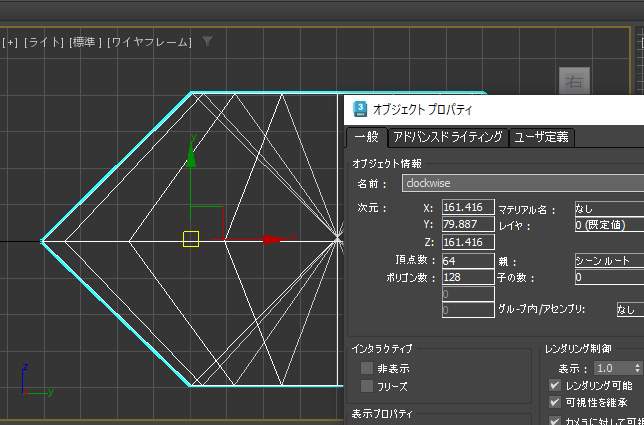
\includegraphics[width=70mm, height=50mm]{no/clockwise.png}
    \end{center}
    \caption{clockwise.png}
    \label{fig:cw}
  \end{minipage}
  \begin{minipage}{0.5\hsize}
    \begin{center}
      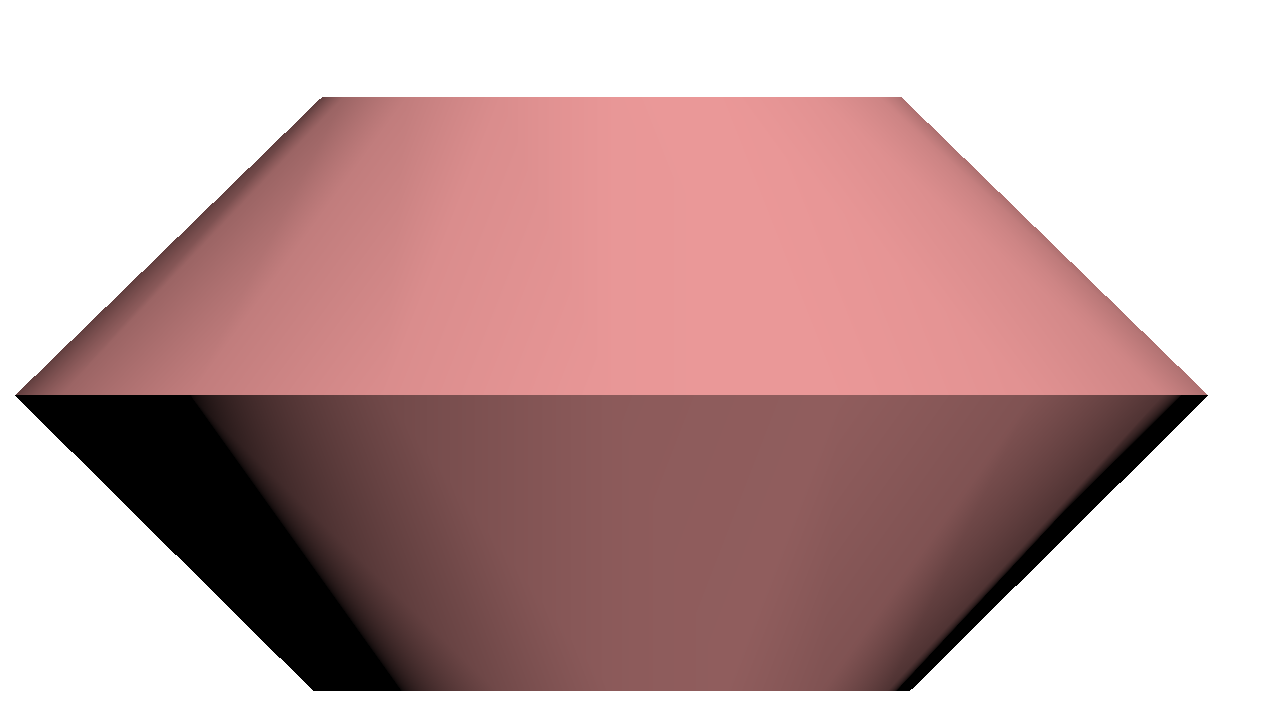
\includegraphics[width=70mm, height=50mm]{no/clockwise-raise.png}
    \end{center}
    \caption{clockwise-raise.png}
    \label{fig:cwa}
  \end{minipage}
\end{figure}
\begin{figure}[htbp]
  \begin{minipage}{0.5\hsize}
    \begin{center}
      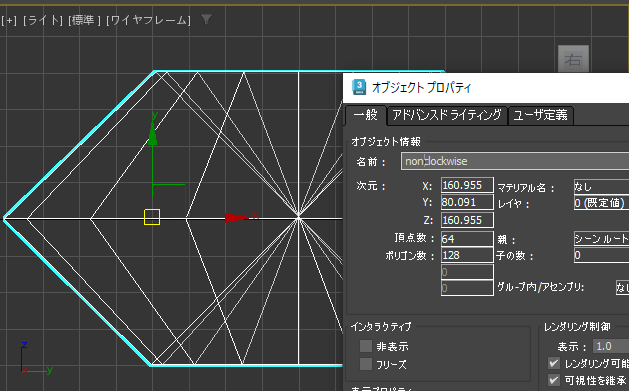
\includegraphics[width=70mm, height=50mm]{no/counterclockwise.png}
    \end{center}
    \caption{counterclockwise.png}
    \label{fig:ccw}
  \end{minipage}
  \begin{minipage}{0.5\hsize}
    \begin{center}
      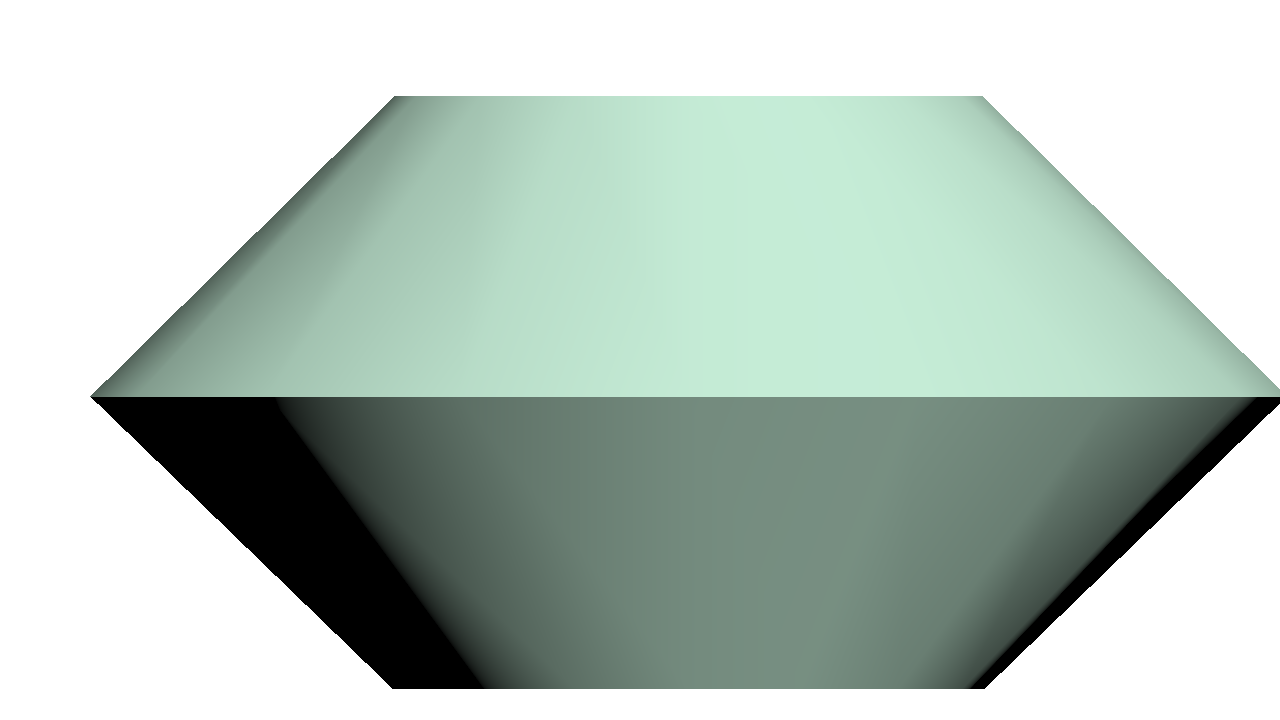
\includegraphics[width=70mm, height=50mm]{no/counterclockwise-raise.png}
    \end{center}
    \caption{counterclockwise-raise.png}
    \label{fig:ccwa}
  \end{minipage}
\end{figure}

\newpage
\section{実験\ 1-2}
スプレインのステップ数を\ 2\ ～\ 20\ に\ 2\ ずつ変更してモデリングした時、概観、ポリゴン数、
レンダリング時間などにどういった差異が出るかを確認しなさい。
\subsection{考察}
%
図\ref{fig:st10}, \ref{fig:st100} を綿密に比較しても差異は見受けられなかった。
ウェブサイト\ iPentec\ によると、スプラインは曲線の滑らかに影響するという\cite{toritchi} 。
裏を返せば、正方形を描いたことで、スプラインの値の高低問わず辺が直線的で、角が直角になったと考えられる。
表\ref{table:1} のポリゴン数は、セグメント数が増加するに連れて増えたことを確認した。
レンダリング時間はステップ数2、20の比較であまり差異が見られなかった。
%

\begin{figure}[htbp]
  \begin{minipage}{0.5\hsize}
    \begin{center}
      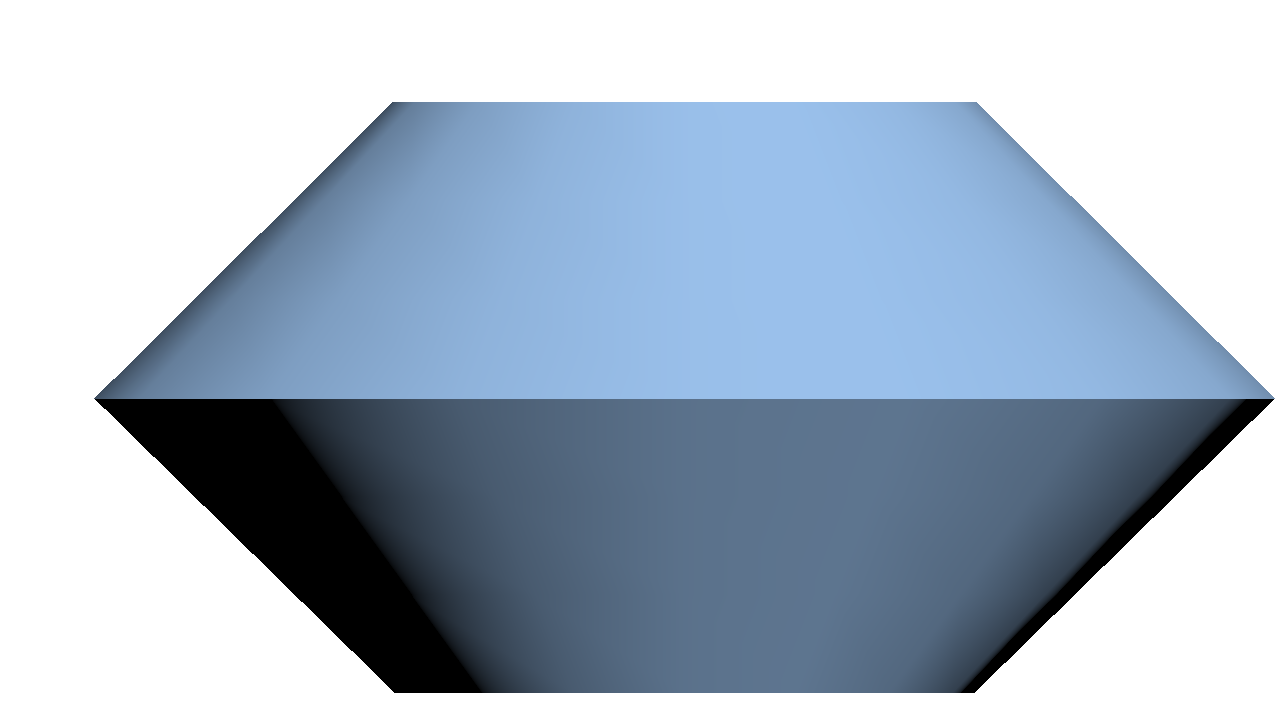
\includegraphics[width=70mm, height=50mm]{no/1-2-2-out.png}
    \end{center}
    \caption{step2.png}
    \label{fig:st10}
  \end{minipage}
  \begin{minipage}{0.5\hsize}
    \begin{center}
      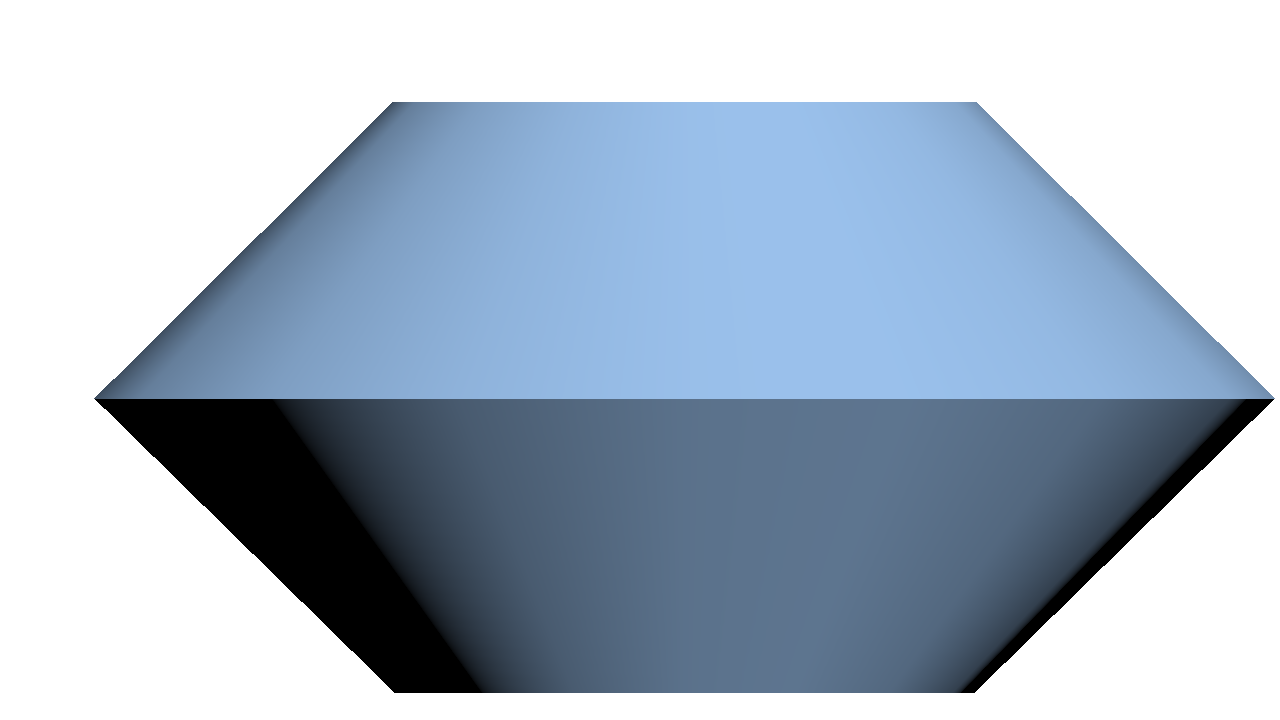
\includegraphics[width=70mm, height=50mm]{no/1-2-20-out.png}
    \end{center}
    \caption{step20.png}
    \label{fig:st100}
  \end{minipage}
\end{figure}

\newpage
\begin{table}
  \centering
  \begin{tabular}{|c|c|c|}
  \hline
  ステップ数 & ポリゴン数 & レンダリング時間\verb|(s)| \\
  \hline
  2 & 13916 & 0.72 \\
  4 & 14172 & 0.72 \\
  6 & 14428 & 0.74 \\
  8 & 14684 & 0.73 \\
  10 & 14940 & 0.85 \\
  12 & 15196 & 0.73 \\
  14 & 15452 & 0.74 \\
  16 & 15708 & 0.74 \\
  18 & 15964 & 0.74 \\
  20 & 16220 & 0.74 \\
  \hline
  \end{tabular}
  \caption{実験\ 1-2}
  \label{table:1}
\end{table}

\newpage
\section{実験\ 1-3}
レイズのセグメント数を\ 10\ ～\ 100\ に\ 10\ ずつ変更してモデリングした時、概観、ポリゴン数、
レンダリング時間などにどういった差異が出るかを確認しなさい。
\subsection{考察}
%
概観の差分は図\ref{fig:s10}, \ref{fig:s100}を見ると明らかであり、前者の外周が\ 10\ の角を持つことから
、後者は恐らく\ 100\ の角を持つのだろう。そのため、概観が滑らかさの観点で異なって見える。
セグメント数とは、レイズの図形回転の頂点を取る回数であり、その対応する頂点同士を
結んでいると考察される。
表\ref{table:2} を分析したところ、セグメント数が増加するに連れて、ポリゴン数も増加している。
ポリゴン数は、\ 3\ Dオブジェクトを構成する面の数であるためである。
\ 4\ ～\ 5\ 桁程度のポリゴン数ではレンダリング時間に与える
影響は少ないとみていいだろう。しかし、演習室で実験を実施した日時が異なると、\ 100\ 枚のレンダリング時間が
表\ref{table:2} のと比較して、30秒程度長くなった。これは、演習室のサーバーの負荷や、
開いているソフトウェアの量、フォーカスされているフレーム等による影響だと考察した。
また、
%
\begin{figure}[htbp]
  \begin{minipage}{0.5\hsize}
    \begin{center}
      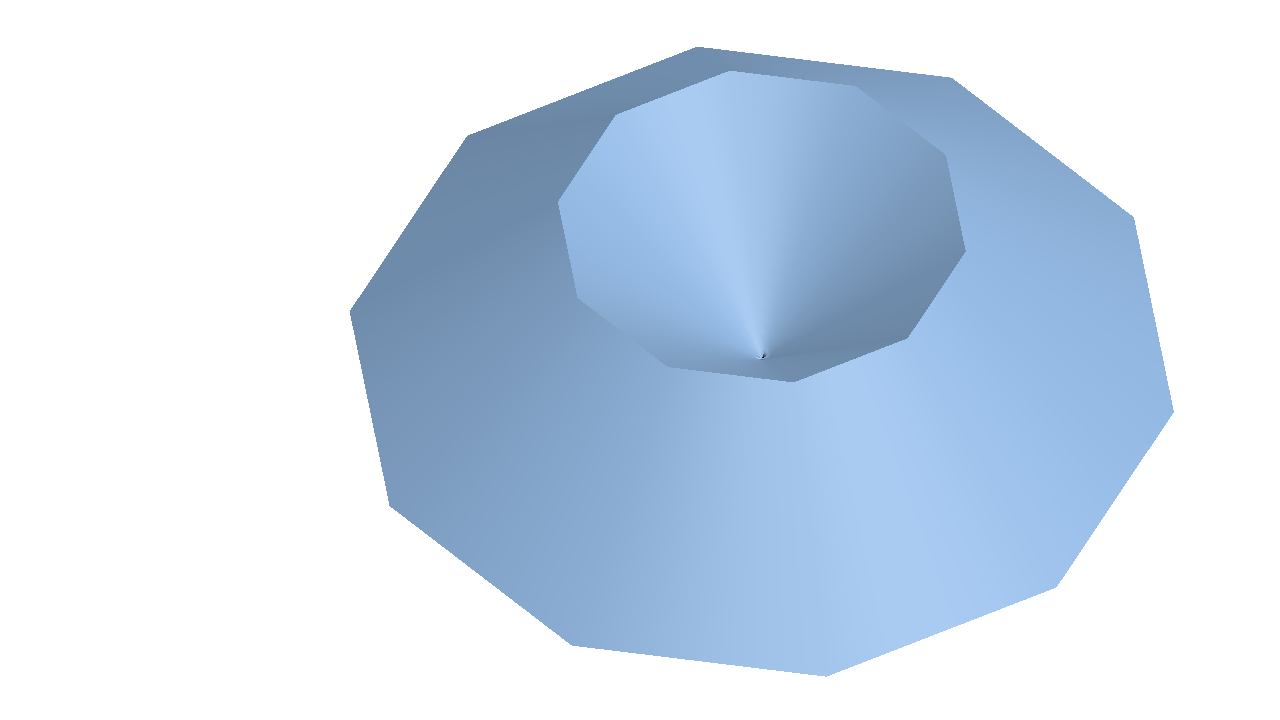
\includegraphics[width=70mm, height=50mm]{no/seg10.png}
    \end{center}
    \caption{seg10.png}
    \label{fig:s10}
  \end{minipage}
  \begin{minipage}{0.5\hsize}
    \begin{center}
      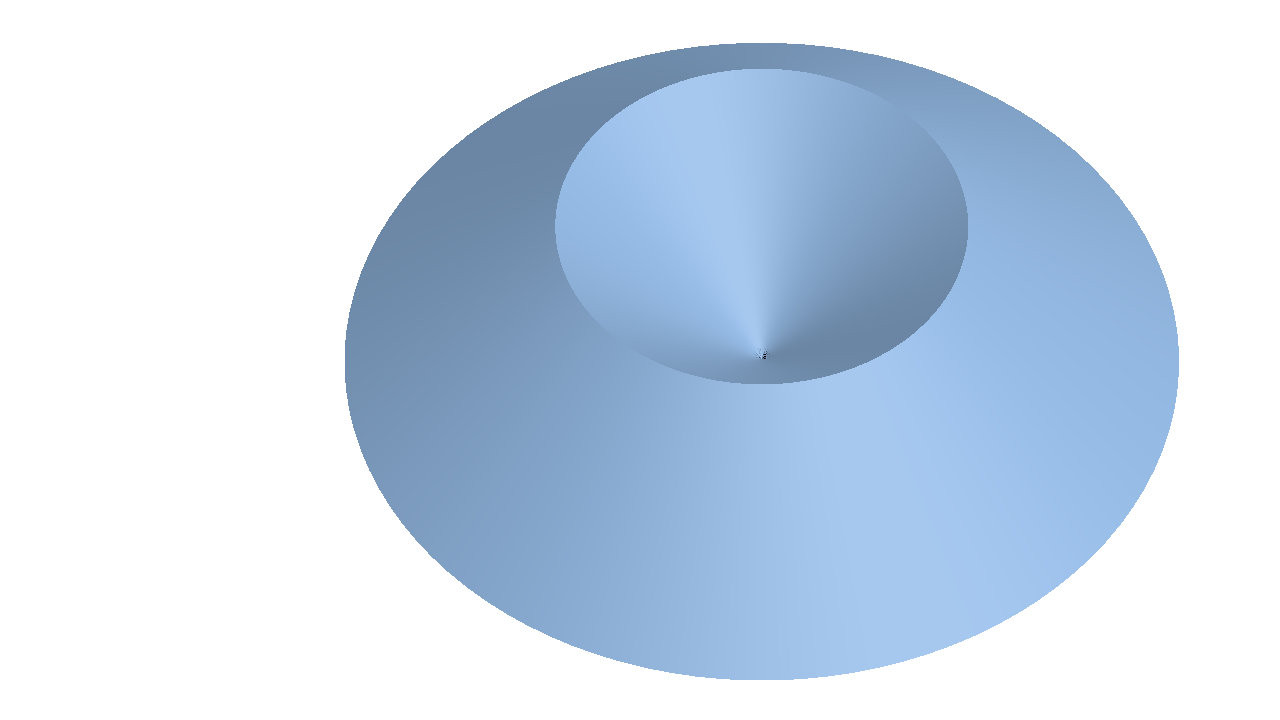
\includegraphics[width=70mm, height=50mm]{no/seg100.png}
    \end{center}
    \caption{seg100.png}
    \label{fig:s100}
  \end{minipage}
\end{figure}

% 表の環境 "\\"は改行。"&"は要素区切り。"|c|c|c|"は要素中央そろえ、縦線で囲む。"\hline"は横線
\newpage
\begin{table}
  \centering
  \begin{tabular}{|c|c|c|}
  \hline
  セグメント数 & ポリゴン数 & レンダリング時間\verb|(s)| \\
  \hline
  10 & 5296 & 0.52 \\
  20 & 6416 & 0.54 \\
  30 & 7536 & 0.53 \\
  40 & 8656 & 0.52 \\
  50 & 9776 & 0.54 \\
  60 & 10896 & 0.55 \\
  70 & 12016 & 0.53 \\
  80 & 13136 & 0.59 \\
  90 & 14256 & 0.58 \\
  100 & 15376 & 0.56 \\
  \hline
  \end{tabular}
  \caption{実験\ 1-3}
  \label{table:2}
\end{table}

\newpage
\renewcommand{\refname}{引用文献}
\begin{thebibliography}{3}
  \bibitem{toritchi}
    とりっち. "描画したスプラインのカーブが滑らかでない (3ds Max の使い方 操作方法 Tips)". iPentec. 2022. \\
    \url{https://www.ipentec.com/document/3ds-max-spline-curve-is-not-smooth}, (参照 2023-11-06).
  \bibitem{Aismiley}
    Aismiley編集部. "AI・人工知能ができること、できないこと。人間にしかできない仕事は？". Aismiley. 2023. \\
    \url{https://aismiley.co.jp/ai_news/what-ai-can-not-do/}, (参照 2023-11-06).
\end{thebibliography}

\renewcommand{\refname}{参考文献}
\begin{thebibliography}{3}
  \bibitem{StudioN9ne}
    StudioN9ne. "S9 Tutorials: 3ds Max Box Modeling Overview". [YouTube Video]. 2010. \\
    \url{https://www.youtube.com/watch?v=_9BaGsMM5GY}, (参照 2023-11-06).
\end{thebibliography}

\end{document}
